\documentclass[aps,pra,reprint,amsmath,amssymb]{revtex4-1}

\usepackage{subfigure,dcolumn}
\usepackage[T2A,T1]{fontenc}
\usepackage[english]{babel}

\usepackage{braket}
\usepackage{graphicx}
\usepackage[colorinlistoftodos]{todonotes}
\usepackage[utf8]{inputenc}

% The following package will be used to typeset the LaTeX codes and is not a necessity to this template
\usepackage{listings}
\lstloadlanguages{[LaTeX]TeX}
\lstset{language=[LaTeX]TeX,keywordstyle=\color{red},showspaces=true,breaklines=true,breakatwhitespace=true,basicstyle=\small\tt,commentstyle=\color{white},frame=single,framerule=0pt,backgroundcolor=\color{yellow}}


\begin{document}


\title{Causality and the N-photon Scattering matrix in waveguide QED}

\author{...}
\affiliation{...}
\email[Corresponding author, ]{The name, complete address, telephone number, and e-mail address of the author to whom correspondence and proofs should be sent.}


\begin{abstract}
The scattering matrix is one of the most fundamental objects for
describing particle processes. It connects the far past state with the
far future state, where the particles are well described by a free
Hamiltonian but they interact in some nontrivial way
for mid times. It can always be split into two parts: the linear part,
where each particle is scattered independently, and the nonlinear one,
which gives information about the interaction among the
particles. Here, we study the linear part of the scattering matrix for
$N$ photons impinging on a local system with several stable states. 
bla, bla
\end{abstract}


\keywords{Quantum optics, scattering matrix, and few-photon photonics.}

\maketitle


\section{Introduction}

{\color{blue}Blablabla on waveguide QED (wQED), scattering matrix as a fundamental object, and causality \cite{weinberg1995,Xu2016}.}


\section{Model in quantum photonics} 

{\color{blue}Hamiltonian and Fig. \ref{fig:input}. Mention it is a chiral model but the generalization to a nonchiral one is trivial \cite{fan10}.}

\begin{figure}
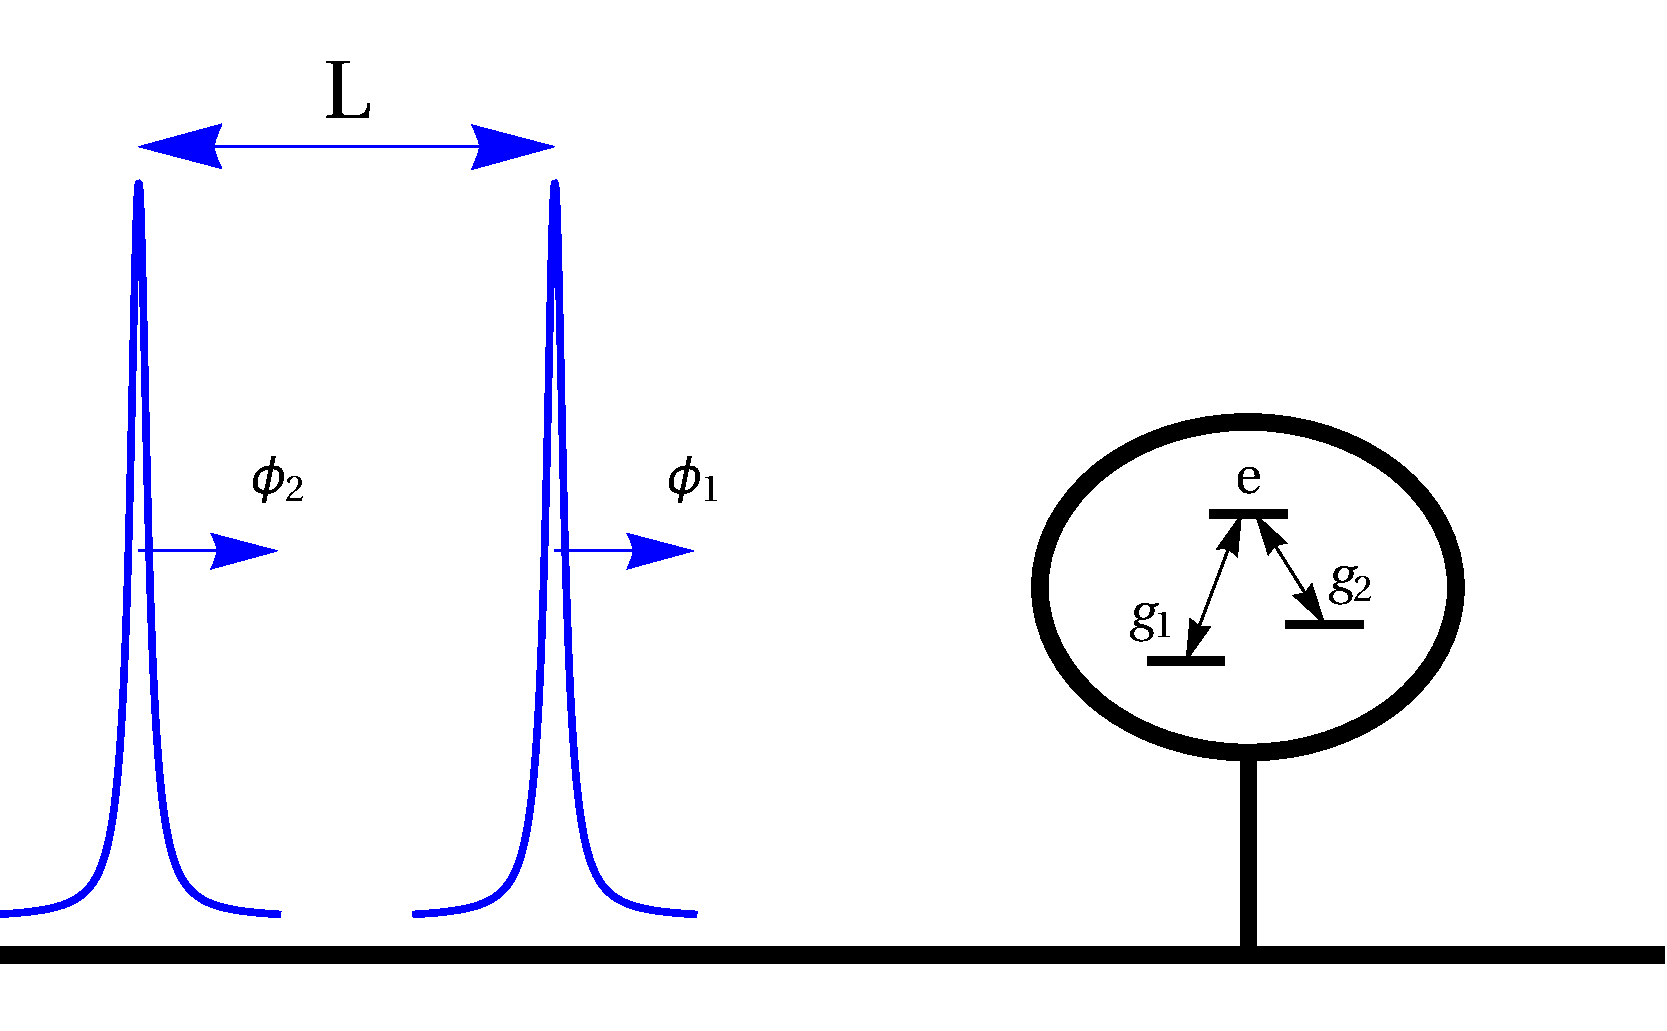
\includegraphics[scale=0.25]{input.pdf}
\caption{Two-photon input state impinging on a $\lambda$ atom. The state $e$ is an unstable state which decays to the stable ones, $|g_1\rangle$ and $|g_2\rangle$.}
\label{fig:input}
\end{figure}

\section{Free-field causality}

{\color{blue}Bounds for the commutators of the free theory.}

\section{Well-defined scattering}

{\color{blue}Conditions required for having well-defined scattering:

\begin{enumerate}
\item ground state $\simeq$ vacuum far enough from the scatterer,
\item free evolution for the fields far enough from the scatterer, and
\item Fig. with decaying ground state.
\end{enumerate}
}

\section{Cluster revisited}

In this section, we build the ansatz for $S^0$ in position space. For the sake of simplicity, we first assume we have two photons. The input photons are placed at $x_1$ and $x_2$ and the outgoing ones are at $y_1$ and $y_2$. The initial and final states for the scatterer are $|g_\nu\rangle$ and $|g_\mu\rangle$, respectively. The ansatz is
\begin{align}\label{eq:S0_2}
(S^0_{y_1y_2x_1x_2})_{\mu\nu}& = \sum_\lambda \overbrace{(S_{y_1x_1})_{\mu\lambda}(S_{y_2x_2})_{\lambda\nu}}^{\text{single-photon process}}\overbrace{\theta(y_2-y_1)}^\text{causality} \nonumber\\
&+ [x_1\leftrightarrow x_2,y_1\leftrightarrow y_2].
\end{align}
As expected from the cluster decomposition principle \cite{weinberg1995}, we take the product of two single-photon $S$ matrices: a photon going from $x_2$ to $y_2$ induces a transition between $|g_\nu\rangle$ and $|g_\lambda\rangle$, and a second photon, which goes from $x_1$ to $y_1$, causes the transition $|g_\lambda\rangle\to |g_\mu\rangle$. Notice there is a summation in the intermediate stable states of the scatterer, $|g_\lambda\rangle$. We multiply this by a step function ($\theta(y)=1$ if $y>0$ and $0$ otherwise) to ensure the outgoing photon placed at $y_2$ leaves the scatterer before the photon at $y_1$. Lastly, we symmetrize the result. The generalization for $N$ photons is straightforward
\begin{align}\label{eq:S0_N}
(S^0_{y_1\dots y_N x_1\dots x_N})_{\mu\nu}& = \sum_{\lambda_1\dots \lambda_{N-1}}\prod_{n=1}^N (S_{y_nx_n})_{\lambda_{n-1}\lambda_n}\nonumber\\
\prod_{m=1}^{N-1}&\theta(y_{m+1}-y_m) + \text{permutations},
\end{align}
with $\lambda_0\equiv \mu$ and $\lambda_N\equiv\nu$. We add all the permutations in $y_n/x_n\leftrightarrow y_m/x_m$ for all $n$ and $m$ in order to symmetrize $S^0$.

We now show the step functions are necessary to fulfil causality. We consider a two-photon input state
\begin{equation}\label{eq:input}
|\Psi_\text{in}\rangle = \frac{1}{\sqrt{2}}(|\phi_1\rangle \otimes|\phi_2\rangle + |\phi_2\rangle\otimes |\phi_1\rangle)\otimes|g_\nu\rangle,
\end{equation}
where $|\phi_n\rangle$ is a single-photon state. The photon whose state is $|\phi_1\rangle$ impinges on the scatterer before the other and they are separated by $L\to\infty$, Fig. \ref{fig:input}. The probability amplitude of going to the state
\begin{equation}
|\Psi_\text{out}\rangle = \frac{1}{\sqrt{2}}(|\phi_{1'}\rangle \otimes|\phi_{2'}\rangle + |\phi_{2'}\rangle\otimes |\phi_{1'}\rangle)\otimes|g_\mu\rangle
\end{equation}
can be computed just with the linear part of the $S$ matrix, since both incident wave packets are highly separated. Taking the ansatz given by Eq. \eqref{eq:S0_2}, this probability amplitude is
\begin{equation}\label{eq:A}
A_{12\to 1'2'}^{\nu\to\mu} \equiv \langle \Psi_\text{out}|S^0|\Psi_\text{in}\rangle =  \sum_\lambda A_{1\to 1'}^{\nu\to\lambda} A_{2\to 2'}^{\lambda\to\mu},
\end{equation}
with $A_{n\to n'}^{\nu\to \mu}\equiv (\langle g_\mu |\otimes \langle \phi_{n'}|)S(|\phi_n\rangle\otimes |g_\nu\rangle)$, that is to say, the probability amplitude for the single-photon process between $|\phi_n\rangle\otimes |g_\nu\rangle$ and $|\phi_{n'}\rangle\otimes |g_\mu\rangle$. We choose $|\phi_{m'}\rangle$ such that $A_{n\to m'}^{\nu\to \mu}=0$ if $n\neq m$. More details on the computation can be found in the Appendix.

Notice this is what one could expect from a standard scattering process: the total amplitude is the product of the amplitudes for both independent process, happening in the proper order. However, if we did not have included the step function in our ansatz, Eq. \eqref{eq:S0_2}, we would have obtained an unphysical term $A_{2\to 2'}^{\nu\to\lambda} A_{1\to 1'}^{\lambda\to\mu}$, which says $|\phi_2\rangle$ impinges on the scatterer before $|\phi_1\rangle$, breaking causality.

Taking the Fourier transform of Eq. \eqref{eq:S0_2}, we can compute $S^0$ in momentum space. Before doing so, the single-photon $S$ matrix in momentum space is
\begin{equation}
(S_{pk})_{\mu\nu}=t_{\mu\nu}(k)\delta(p+E_\mu-k-E_\nu),
\end{equation}
with $k$ and $p$ the incident and outgoing momenta, respectively, and $|g_\nu\rangle$ and $|g_\mu\rangle$ the initial and final states of the scatterer. The energies $E_\nu$ and $E_\mu$ correspond to the states $|g_\nu\rangle$ and $|g_\mu\rangle$. The factor $t_{\mu\nu}(k)$ is the so-called transmission amplitude. Notice that the Dirac delta guarantees energy conservation {\color{blue}WE HAVE TO MENTION SOMEWHERE $v_g=1$}. Then, the two-photon $S^0$ matrix is
\begin{align}\label{eq:S0_2p}
(S_{p_1p_2k_1k_2}^0)_{\mu\nu}=&\frac{1}{(2\pi)^2}\int  dy_1dy_2dx_1dx_2\; (S_{y_1y_2x_1x_2}^0)_{\mu\nu}\nonumber\\
& e^{-i(p_1y_1+p_2y_2)}  e^{i(k_1x_1+k_2x_2)} \nonumber\\
=  \frac{i}{2\pi}\sum_{n,m=1}^2 &\sum_\lambda  \frac{t_{\mu\lambda}(k_n) t_{\lambda\nu}(k_{\overline{n}})}{p_m+E_\mu -k_n -E_\lambda + i0^+}\nonumber\\
&\delta(p_1+p_2+E_\mu - k_1-k_2-E_\nu).
\end{align}
Here, $\overline{n}\neq n$, \emph{e.g.}, $\overline{n}=2$ if $n=1$. This structure has recently been found by Xu and Fan in \cite{Xu2016} for a $\lambda$ atom, a three-level atom which has two stable states and one unstable state, see the scatterer of Fig. \ref{fig:input}. This is not what one finds for wQED systems if the stable state of the scatterer is unique \cite{fan10,Rephaeli2011,Sanchez-Burillo2016}, as shown in general in \cite{xu13}. In that kind of system, there are two Dirac deltas, one for the energy conservation of each photon. In our case, the global Dirac delta imposes energy conservation of the whole process, but each photon does not conserve its energy individually in general. %However, for an input state such as \eqref{eq:input}, both photons do conserve its energy individually. The denominator of Eq. \eqref{eq:S0_2p} comes from the Fourier transform of $\theta$ and it is related to the order in which both photons interact with the scatterer.

If there is an only stable state, one can trivially show $S^0$ in position space is \eqref{eq:S0_2}
\begin{equation}
S^0_{y_1y_2x_1x_2} = S_{y_1x_1}S_{y_2x_2} + S_{y_1x_2}S_{y_2x_1}.
\end{equation}
Notice the step function has disappeared. This gives the double Dirac delta structure in momentum space.

{\color{blue} Conditions for the commutator $[a_\text{out}(t),a_\text{in}^\dagger(t')]$ so that $A_{12\to 1'2'}^{\nu\to\mu} = \sum_\lambda A_{1\to 1'}^{\nu\to\lambda}A_{2\to 2'}^{\lambda\to\mu}$ is true \cite{Xu2015}.
}

\section{Examples}

{\color{blue}
\begin{enumerate}
\item $\lambda$ atom with $N=2$ in momentum space \cite{Xu2016}. Fluorescence from the new part of $S^0$. How the fluorescence decays.
\item Ultrastrong MPS. Fig. with resonance fluorescence. We might include a figure with the decay of the fluorescence as a function of $L$. \cite{Sanchez-Burillo2014,Sanchez-Burillo2015}.
\end{enumerate}
}

\section{Summary and acknowledgements}

\appendix

\section{$S^0$ in momentum space}\label{app:Sp}

{\color{blue}
\begin{enumerate}
\item Computation in general: Figs. \ref{fig:lower} and \ref{fig:upper}.
\item To particularize for $N=2$ and $\lambda$ atom \cite{Xu2016}.
\end{enumerate}
}

\begin{figure}[tbh!]
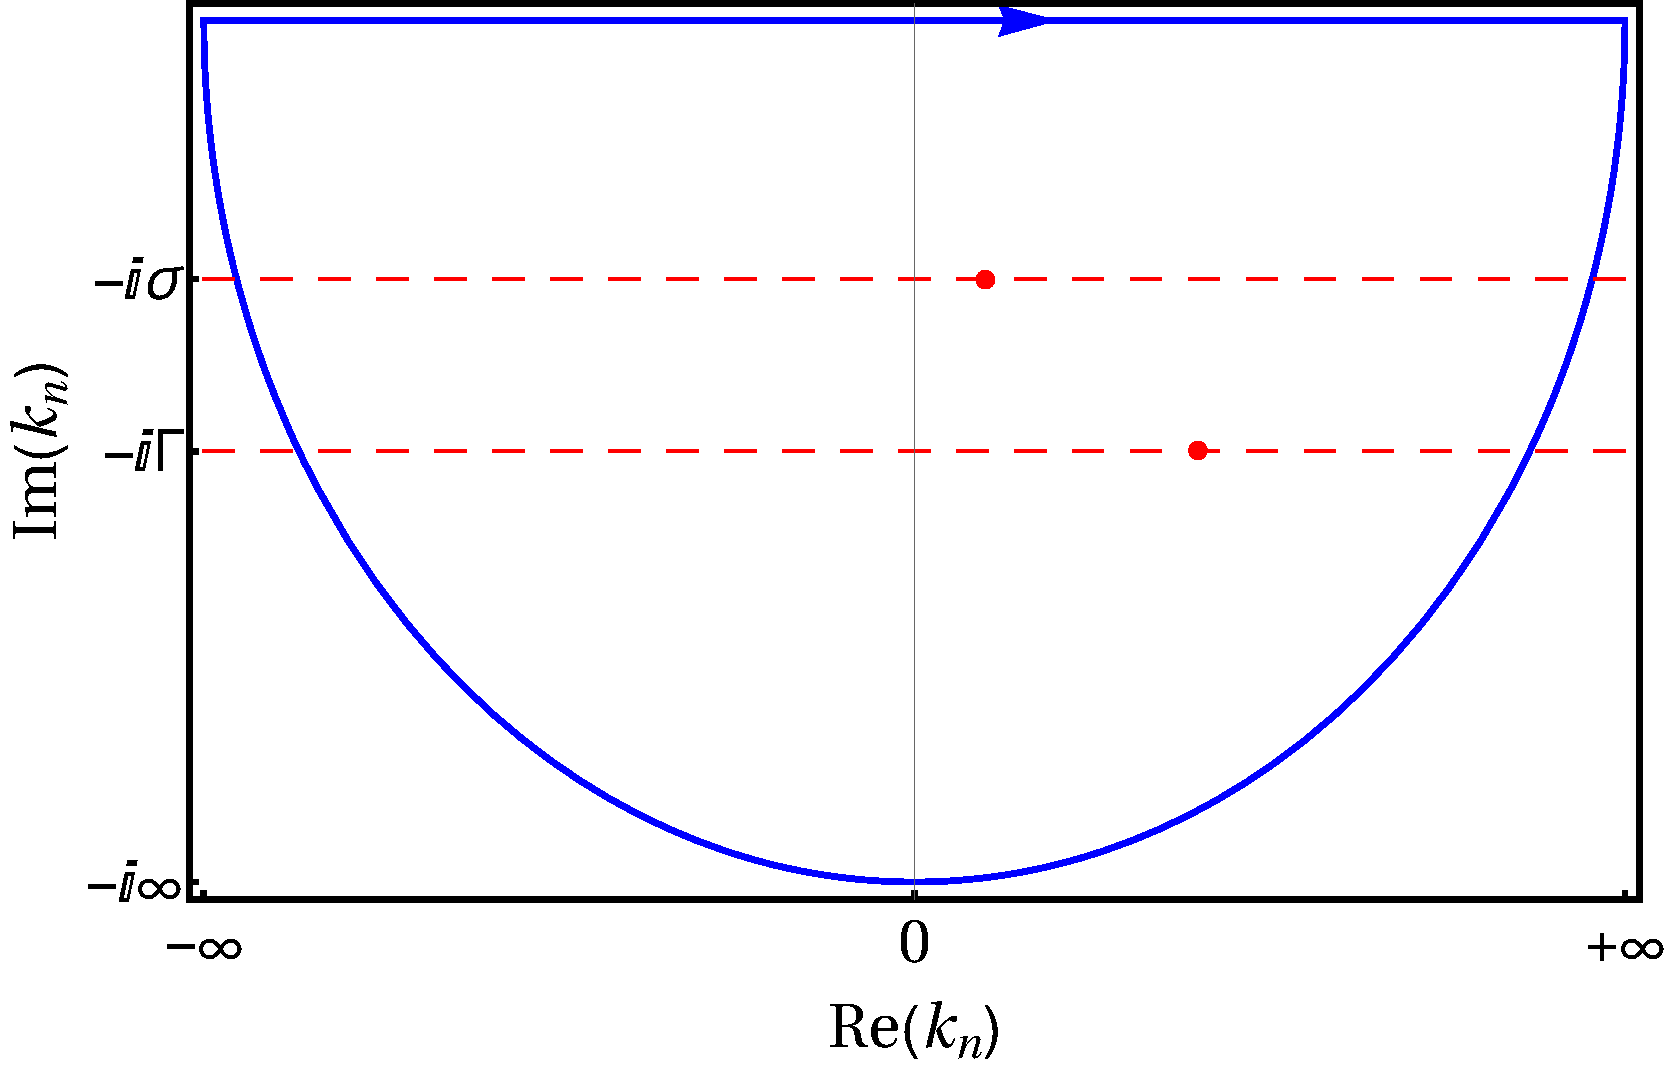
\includegraphics[scale=0.25]{lower_contour.pdf}
\caption{Integration contour for Eq. (...). The red points are the poles of the
integrand. The values of the real parts are arbitrary.}
\label{fig:lower}
\end{figure}

\begin{figure}[tbh!]
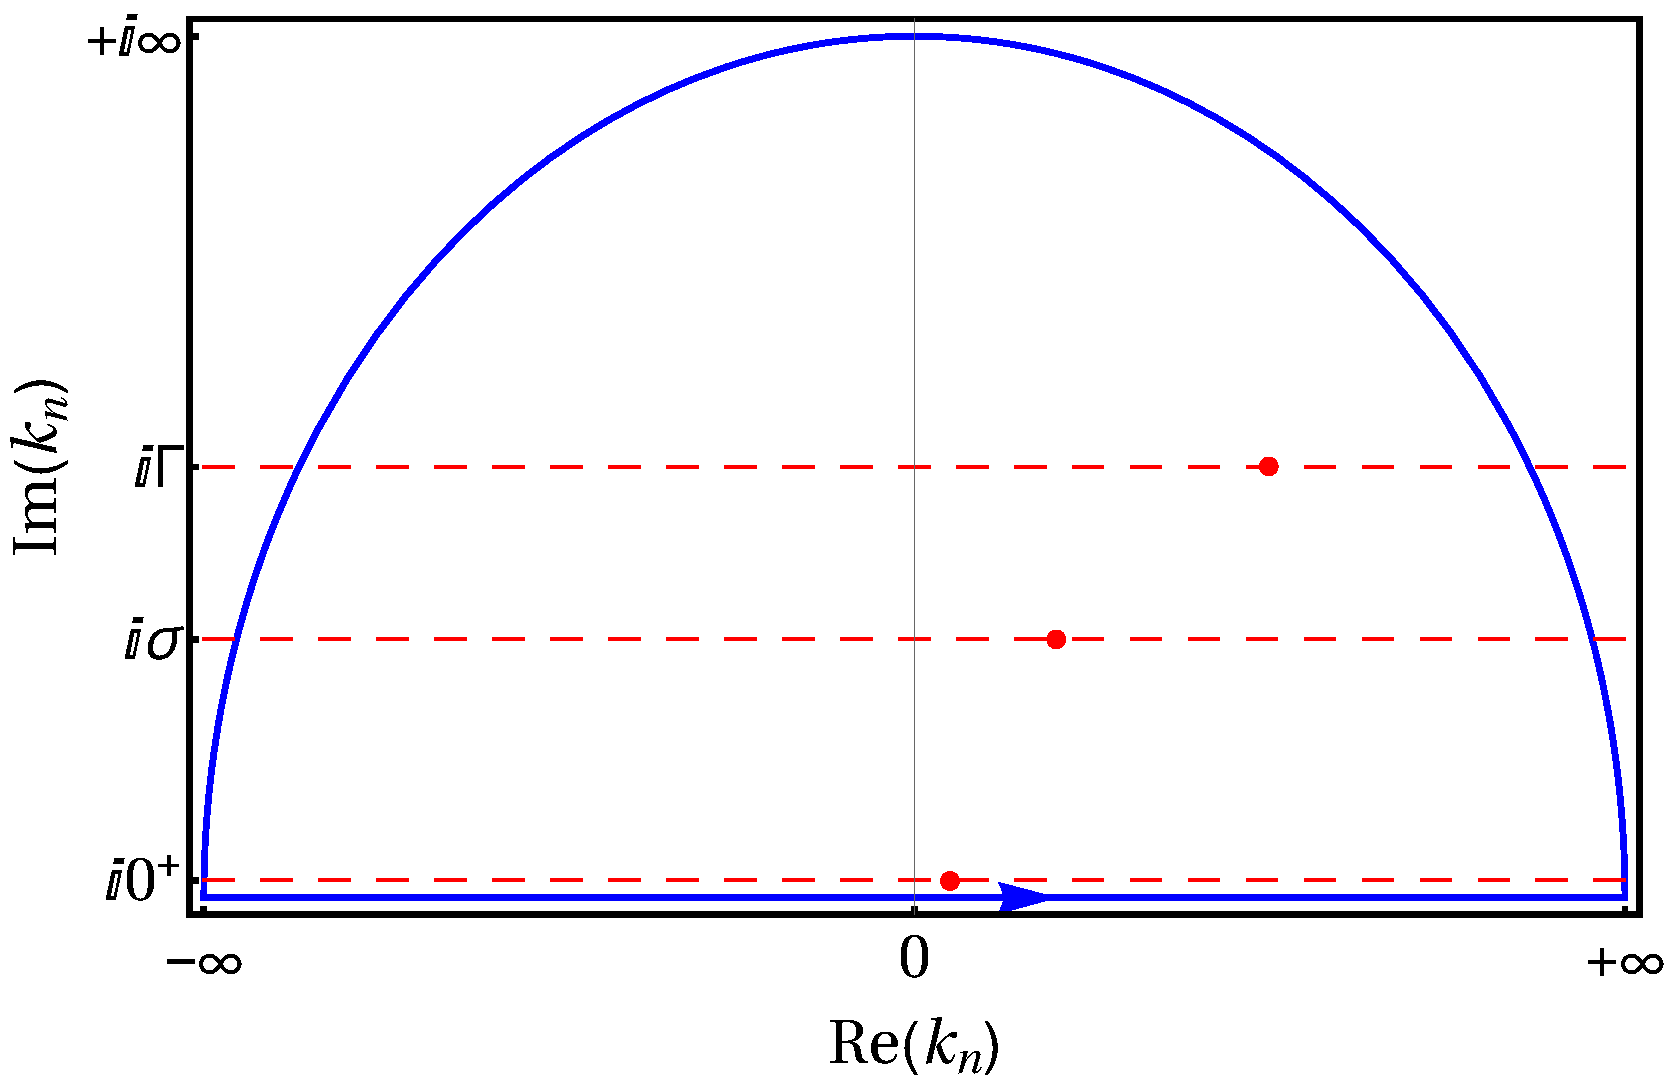
\includegraphics[scale=0.25]{upper_contour.pdf}
\caption{Integration contour for Eq. (...). The red points are the poles of the
integrand. The values of the real parts are arbitrary.}
\label{fig:upper}
\end{figure}

\section{Scattering amplitude}\label{app:A}

{\color{blue}Computation of the scattering amplitude Eq. \eqref{eq:A}.}

\section{Matrix Product States}\label{app:mps}

{\color{blue}
Brief summary of MPS and how to apply them to few-photon photonics problems.}

\bibliographystyle{apsrev4-1}
\bibliography{bib_cluster}



\end{document}